\documentclass{standalone}
\usepackage{tikz}
\pagestyle{empty}

\begin{document}
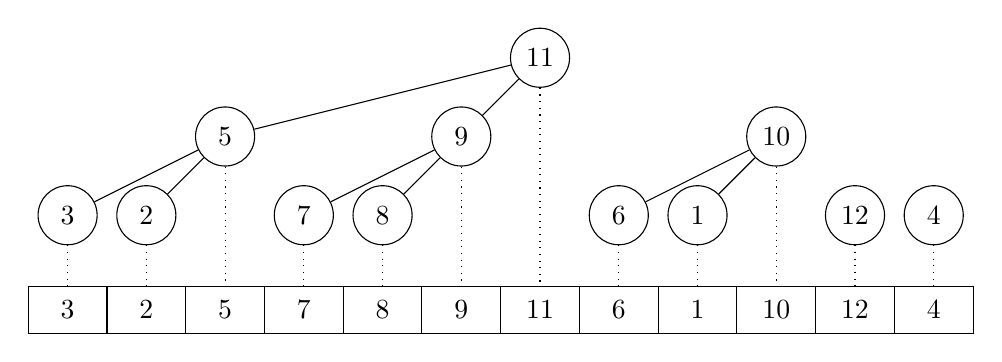
\begin{tikzpicture}

\tikzstyle{every node}=[draw,shape=circle,minimum size=0.75cm];

% Draw the poplar heap nodes
\node (n1) at (0,0) {3};
\node (n2) at (1,0) {2};
\node (n3) at (2,1) {5};
\node (n4) at (3,0) {7};
\node (n5) at (4,0) {8};
\node (n6) at (5,1) {9};
\node (n7) at (6,2) {11};
\node (n8) at (7,0) {6};
\node (n9) at (8,0) {1};
\node (n10) at (9,1) {10};
\node (n11) at (10,0) {12};
\node (n12) at (11,0) {4};

% Links between the nodes
\draw (n7) -- (n6)
(n7) -- (n3)
(n6) -- (n5)
(n6) -- (n4)
(n3) -- (n2)
(n3) -- (n1)
(n10) -- (n9)
(n10) -- (n8);

% Draw the array representation of the poplar heap 
\tikzstyle{every node}=[draw,shape=rectangle,minimum width=1cm,minimum height=0.6cm,anchor=center];
\foreach \x [count=\idx] in {3,2,5,7,8,9,11,6,1,10,12,4}
  \node (r\idx) at (\idx-1,-1.2){\x};

% Explicitly link the nodes to the array representation
\foreach \x in {1,...,12}
   \draw[dotted] (n\x) -- (r\x);

\end{tikzpicture}
\end{document}
